\documentclass[type = bachelor]{whu-thesis}
\usepackage{textcomp,mathcomp}
\usepackage{siunitx}
\usepackage{chemfig}
\usepackage{graphicx}

\whusetup
  {
    info               =
      {
        title          = {金刚石氮-空位色心的\\电荷态调控和性质表征},
        title*         = {Modulation of Charge States and Characterization of Properties\\ in Nitrogen-Vacancy Centers of Diamond},
        student-number = {2020302192129},
        school         = {弘毅学堂},
        author         = {邹迪玮},
        author*        = {Diwei Zou},
        subject        = {学科},
        major          = {微电子科学与工程},
        advisor        = {周利 , 副教授;孙启超 , 研究员},
        direction      = {研究方向},
        date           = {2024/5},
        keywords       = {关键词 1 , 关键词 2 , 关键词 3 , 关键词 4 , 一个非常非常,非常非常长——的关键词 5},
        keywords*      = {key word 1 , key word 2 , key word 3 , key word 4 , {and a very very, very very long key word---the key word 5}},
      },
    style              =
      {
        graphics-path  = {{figures/}{data/}},
        list-of-figures,
        list-of-tables,
      },
    element            =
      {
        innovation     = {pages/innovation},
        abstract       = {pages/abstract},
        abstract*      = {pages/enabstract},
        bibliography   = {ref/refs_1}
      }
  }
\begin{document}

% Chapter 1

\chapter{金刚石中的氮-空位色心}

\section{金刚石}
金刚石是碳元素的一种常见的同素异形体,在晶体结构上,每一个碳原子被周围的四个碳原子包围并与之形成共价键,从而形成四面体的面心立方结构的晶体。金刚石中的碳原子紧密结合在一起,这样特殊的晶体结构和原子之间稳定的键合方式使得金刚石拥有很多物理和化学上的优异性质,如高硬度、高热导率、高折射率、高抗压强度、高化学稳定性、高电阻率、低热膨胀系数、低摩擦系数、低表面粗糙度、低吸附性等。这些优异的性质使得金刚石在很多领域都有着广泛的应用,如磨料、切割工具、磨料涂层、磁头、光学窗口、高功率激光器件、高频电子器件、生物医学器件等。

金刚石是最坚硬的天然形成的物质,其机械硬度高达 10000 \unit{\kilogram\per\milli\meter\squared},德拜温度高达1860 \unit{\kelvin},它的杨氏模量为1050 \unit{\GPa},有着22 \unit{\watt\per\centi\meter\per\kelvin}的热导率、较低的热展宽系数、较高的击穿电场强度(> 10 \unit{\mega\volt\per\centi\meter}),以及较强的载流子迁移率(对于电子为4500 \unit{\centi\meter\squared\per\volt},对于空穴为3800 \unit{\centi\meter\squared\per\volt})。对于纯净的金刚石而言,其密度为$\rho =$ 3.52 \unit{\g\per\cm},折射率$n =$ 2.39,同时有5.47 \unit{\electronvolt}的较宽带隙,这使其投射光谱范围非常广,从紫外波段(Ultraviolet, UV)到近红外波段(Near Infrared, IR)都可以覆盖到,外观高度透明纯净,拥有极高的透光率 \cite{mildren2013optical, lonvcar2013quantum}。

金刚石在结构上的稳定性使得其化学性质非常的不活跃,因此它几乎不能和大部分化学物质发生反应。所以金刚石有着极低的细胞毒性,使得其在生物、医学领域有着广泛的应用 \cite{schirhagl2014nitrogen,wu2016diamond}。同时,金刚石的化学稳定性也使得其在高温、高压、强腐蚀性环境下有着很好的稳定性,因此金刚石也被广泛应用于高温、高压、强腐蚀性环境下的传感器、探测器等器件中 \cite{umezawa2012high, jayaraman1983diamond}。

由于金刚石晶体的结构非常的整齐和规则,在自然情况下,只有很少一部分的杂质会存在于金刚石晶体中,并参与形成晶格结构。自然界中常见的最主要的金刚石中的杂质是氮和硼元素,因此金刚石可以根据杂质的种类和含量分为不同的类型,主要有两种大类:type \uppercase\expandafter{\romannumeral1}和type \uppercase\expandafter{\romannumeral2},在其中又可以分为四个子类:type \uppercase\expandafter{\romannumeral1}a、type \uppercase\expandafter{\romannumeral1}b、type \uppercase\expandafter{\romannumeral2}a、type \uppercase\expandafter{\romannumeral2}b \cite{breeding2009type}。在这些分类中,type \uppercase\expandafter{\romannumeral1}型的金刚石中主要含有氮元素杂质,type \uppercase\expandafter{\romannumeral1}a型金刚石中的氮元素含量较高,最多有3000 ppm(parts per million,即百万分之一);而type \uppercase\expandafter{\romannumeral1}b型金刚石中的氮元素含量稍低,一般情况下不到500 ppm。由于空气中广泛存在的氮气和土壤中各种各样的氮元素,在自然界中形成的金刚石通常为type \uppercase\expandafter{\romannumeral1}a或者\uppercase\expandafter{\romannumeral1}b。对于type \uppercase\expandafter{\romannumeral2}型的金刚石而言,氮元素的含量远远小于type \uppercase\expandafter{\romannumeral1}型金刚石,通常低于20 ppm。其中,type \uppercase\expandafter{\romannumeral2}b型金刚石中的硼元素杂质含量要高于type \uppercase\expandafter{\romannumeral2}a型。Type \uppercase\expandafter{\romannumeral2}型金刚石的含量极其稀少,而且很少能在自然界中被发现。在科学研究中,type \uppercase\expandafter{\romannumeral2}型金刚石由于其晶体纯净的性质,有着各种各样独特的应用场景。对于科学研究而言,为了保证金刚石样品性质的一致性和实验的可重复性,高纯度和可控掺杂的人造金刚石生长合成技术应运而生 \cite{sumiya1997crystalline, spitsyn1981vapor, gracio2010diamond}。

\subsection{人工合成生长金刚石}
目前主流的人造金刚石样品合成技术主要分为两种,一种是高温高压方法(High Pressure High Temperature,HPHT)和化学气相沉积法(Chemical Vapor Deposition, CVD)。对于HPHT方法而言,其原理主要是模仿天然金刚石在地壳中的形成过程,将碳元素另一种常见的同素异形体石墨的晶体结构在极端的超高温超高压环境下(温度在\SI{1400}{\degreeCelsius}左右,压强在\SI{5.5}{\GPa}左右),通过金属触媒粉的催化作用,转换成具有$sp^3$杂化轨道的金刚石晶体结构 \cite{dossa2023analysis}。HPHT方法使得人类可以在工业上大规模高效率地生产type \uppercase\expandafter{\romannumeral1}型金刚石,但是由于空气中大量的氮气存在,HPHT方法难以生产高纯度低杂质含量的type \uppercase\expandafter{\romannumeral2}型金刚石。由此,为了制备高纯度和可控掺杂的实验级金刚石样品,化学气相沉积的方法逐渐受到科学家们的关注和广泛使用。

CVD方法是一种铜质外延的生长过程,需要在金刚石晶种基面上生长新的金刚石\cite{isberg2002high,isberg2002high}。因此,对于生长出来的晶体,其质量主要取决于晶种的种类和取向,而在非金刚石晶种表面生长会导致生长出有许多单晶金刚石各向同性紧密结合形成的多晶金刚石晶体\cite{mildren2013optical, jahnke2012long}。如果想要形成科学实验中可用的单晶金刚石,就必须用单晶金刚石作为晶种来进行CVD生长。在实际生长的过程中,科学家们通常用{100}取向的晶种衬底来保证尽可能少的生长缺陷\cite{gicquel2001cvd}。

在CVD方法生长金刚石的过程中,除了晶种之外,碳元素源也是比较重要的一个因素。通常情况下,碳元素主要来自于烃类气体,甲烷\chemfig{CH_4}和氢气\chemfig{H_2}的混合气体就是在实验合成的过程中较为理想易得的碳源。对于CVD生长金刚石的过程而言,这些碳源气体需要通过不同的方法来激活,常见的方法有通过热丝(hot filament)或者微波等离子体(microwave plasma),其中微波等离子体气相沉积(Microwave Plasma Chemical Deposition, MPCVD)的方法是生长type \uppercase\expandafter{\romannumeral2}型金刚石最有效的方法\cite{robins1990line, nemanich2014cvd}。在微波等离子体激活后,碳源气体内部形成许多高度反应性的自由基(reactive radicals),活跃的氢自由基(H$\cdot$)有两个重要的功能,一个是终止了已经生长的金刚石表面,从而防止具有$sp^2$杂化轨道的石墨碳原子;其次氢原子可以刻蚀掉已经生成的具有$sp^2$杂化轨道的石墨碳原子,从而在晶种沉底表面上提供悬垂的$sp^3$化学键,使其能够和已经极化的甲基自由基(CH$_3\cdot$)轻松结合,使得单晶金刚石能在沉底表面逐渐生长\cite{denisenko2010surface}。在生长的过程中,各种参数同样十分重要,例如生长腔内压强、温度、气体流速、微波功率等因素决定了生长出来的金刚石的各种性质,使其适用于不同的应用场景。本人于2021年的时候提出了一种n型共掺杂金刚石半导体材料制备的多尺度耦合仿真方法,通过宏观-介观-微观三个尺度的相互耦合,调整MPCVD方法生长金刚石过程中的各种参数,来提高特定用途金刚石的生长合成效率\cite{CN113096749B}。

\subsection{金刚石晶体结构}
金刚石晶体是由每个碳原子和周围四个相邻的碳原子结合,生成四个共价键组成的正四面体结构,其晶格常数为$a_0 = 3.567$ \unit{\angstrom}。金刚石晶体可以看成是两个面心立方晶体的嵌套,其中一个面心立方晶体在三维空间的三个轴上上相对于另一个移动了$\frac{a_0}{4}$,原点从$(0, 0, 0)$移动到了$(\frac{a_0}{4}, \frac{a_0}{4}, \frac{a_0}{4})$。这样的晶体结构使得金刚石非常的坚硬,每一个晶胞中包含着8个碳原子,每一个碳原子的核外电子都呈现$sp^3$杂化轨道结构,和相邻的四个碳原子形成长度为1.44 \unit{\angstrom}的共价键,它的晶体结构见图 \ref{fig: Diamond Lattice}所示。

\begin{figure}[h]
  \centering
  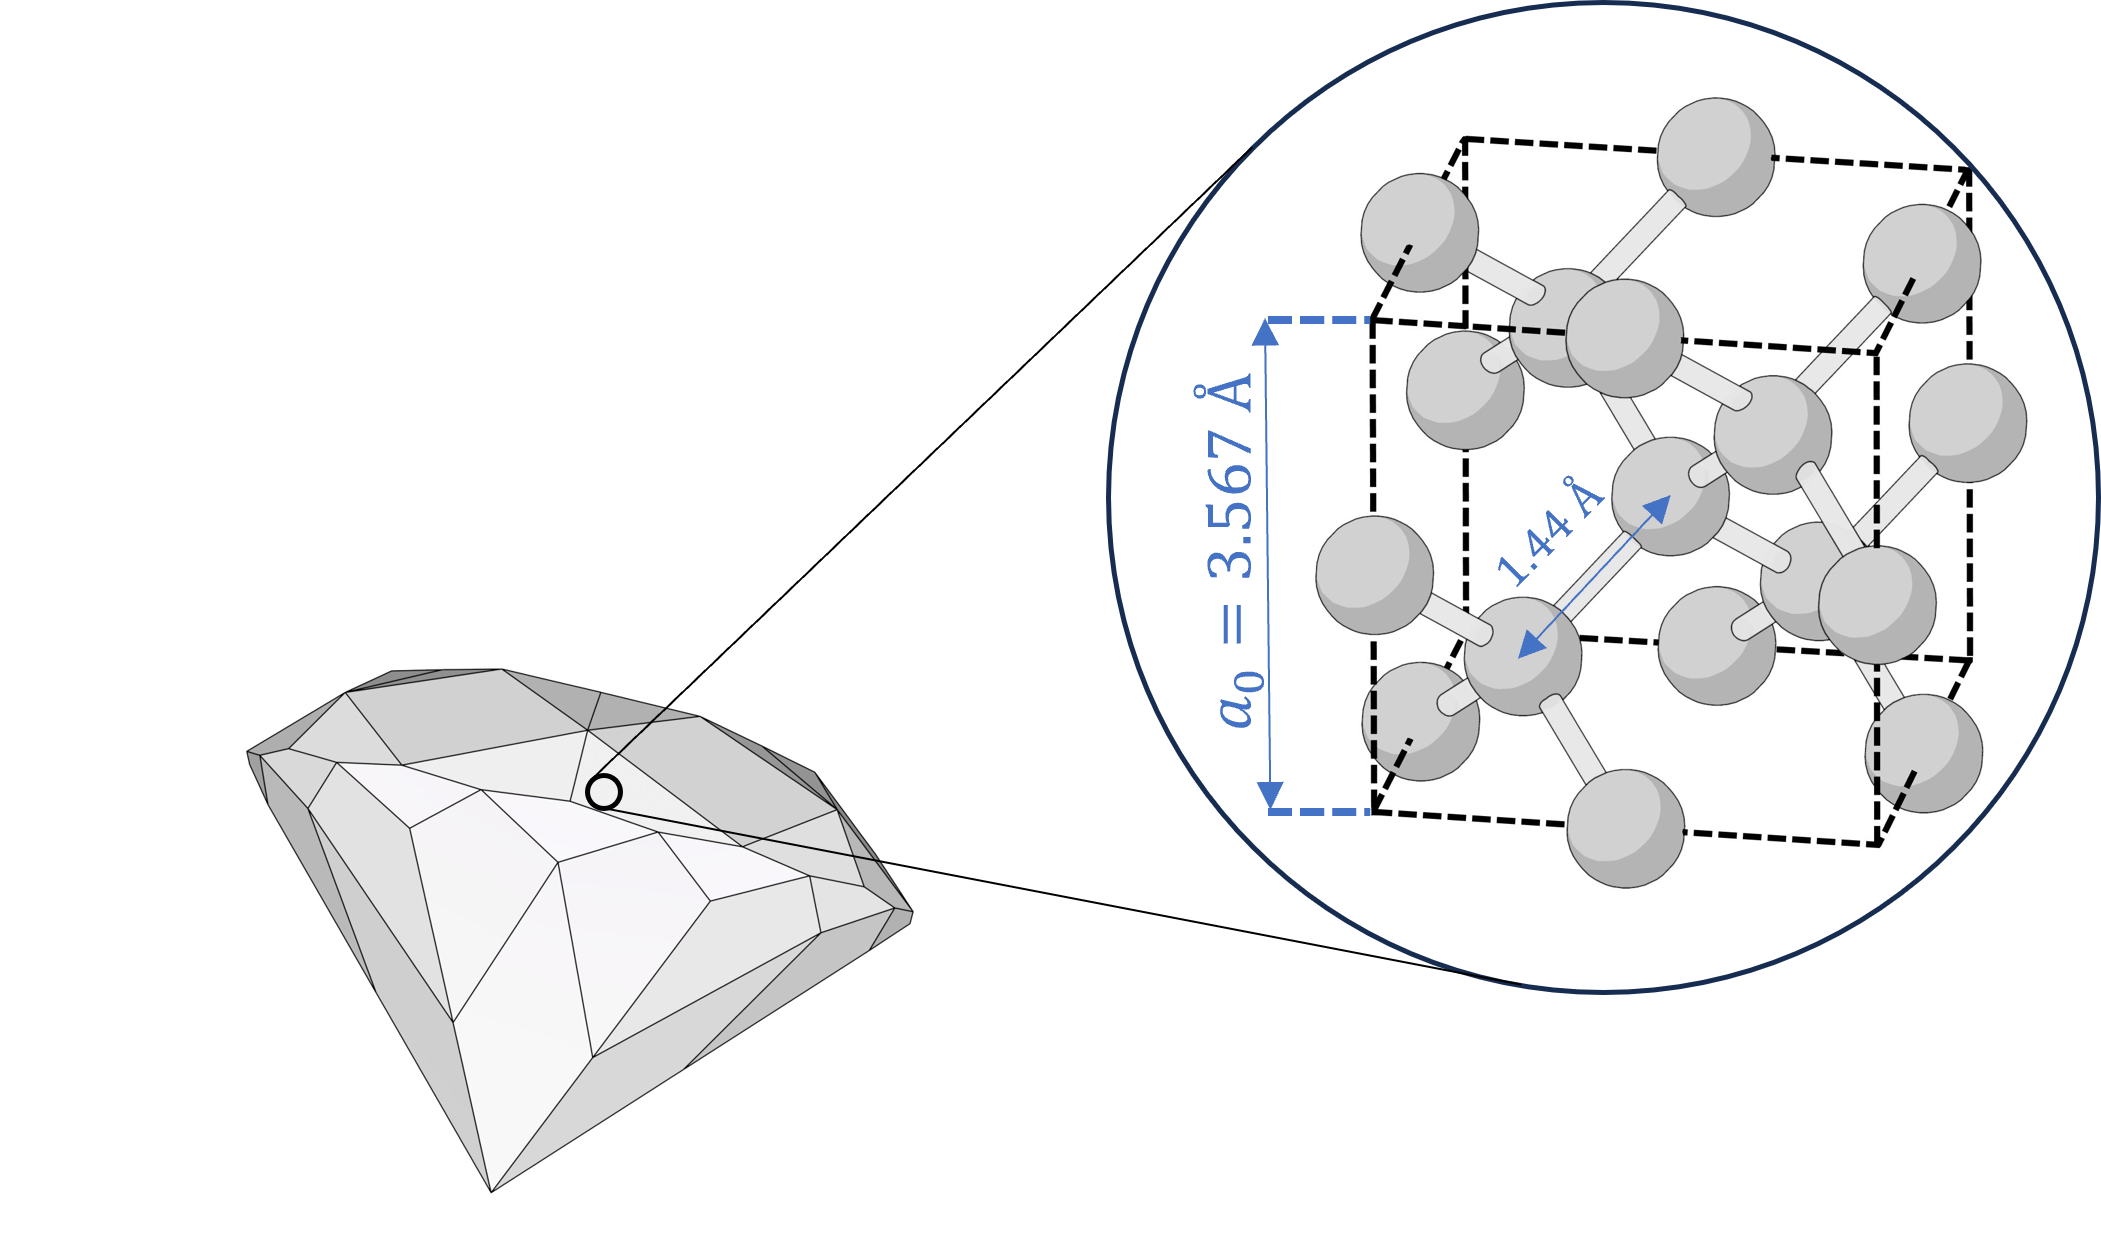
\includegraphics[width=0.9\textwidth]{figures/Chapter 1/Diamond Lattice.png}
  \caption[金刚石及其晶胞结构]{金刚石及其晶胞结构}
  \label{fig: Diamond Lattice}
\end{figure}

然而,在金刚石晶体合成或生长的过程中,晶格缺陷会不可避免的出现,它们会对金刚石的性质产生各种各样的影响,尤其是电子结构产生较大的影响\cite{jelezko2006single, nebel2003electronic}。金刚石晶体中最常见的晶格缺陷是空位(vacancy),这是一种本征晶格缺陷,源于金刚石的中的单个碳原子在其原本的晶格结构上的缺失,每一个孤立的空位可以吸收741 nm的光子,有着高浓度空位的金刚石在一定条件下会呈现蓝绿色的色调,因此金刚石晶体结构中的空位缺陷也被称为色心(color centers),如图 \ref{fig: Color Center}所示\cite{waldermann2007creating, kiflawi2007electron}。

\begin{figure}
  \centering
  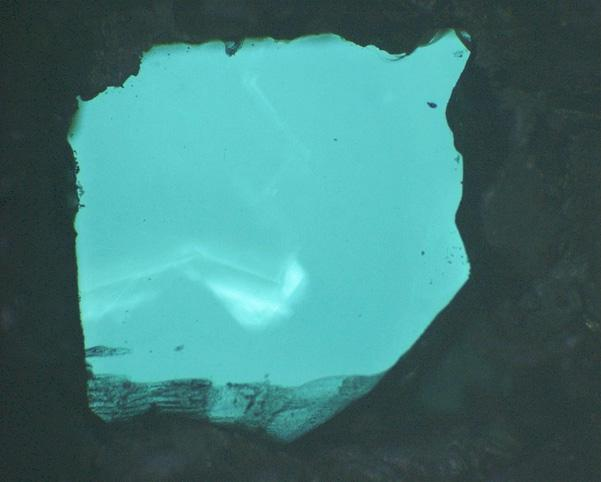
\includegraphics[width=0.7\textwidth]{figures/Chapter 1/Color Center.jpg}
  \caption[电子辐照的type \uppercase\expandafter{\romannumeral1}a型金刚石样品显微图片]{电子辐照的type \uppercase\expandafter{\romannumeral1}a型金刚石样品显微图片。浅色区域的空位和氮浓度较低,样品尺寸为\(1\times1\times0.5 \, \mathrm{mm^3}\)。}
  \label{fig: Color Center}
\end{figure}

\subsection{金刚石色心}
金刚石是一种宽禁带半导体,实验上测得其价带(valence band,VB)和导带(conduction band,CB)之间的带隙宽度大约为5.5 \unit{\eV} \cite{mildren2013optical,cheng2023bandgap,wort2008diamond}。尽管纯净的金刚石呈现无色透明的质地,可以透过的波长范围从UV到IR,但是由于晶格中存在的缺陷或者杂质,使得金刚石体系的带隙之中会出现额外的能级结构,其中的一些能级结构具有活跃的光学性质。因此,这些缺陷结构可以吸收可见光,并在缺陷浓度足够高的时候,使得金刚石材料呈现出特定的颜色,比如高浓度的硼元素会使金刚石呈现蓝色,镍元素相关的缺陷会让金刚石呈现棕色。目前人类已知金刚石中的涉及到光学跃迁性质的荧光缺陷有超过100种,这些缺陷都可以被称为色心\cite{koizumi2008physics,jelezko2006single}。许多的色心都和氮元素杂质有关,因为氮元素是金刚石中最常见的元素,高浓度的氮元素掺杂会使得金刚石呈现黄色的色泽\cite{breeding2020naturally, zaitsev2016spectroscopic}。

金刚石色心种的缺陷能级和电子结构之间的光学跃迁过程可以被人为地进行激光调控,在这个过程中会有不同的激发机理,取决于色心相关的缺陷能级的性质,如图 \ref{fig: Optical Transition}所示。比如,激光的光子可以将缺陷能级的电子激发到导带之中(见图1.3a \uppercase\expandafter{\romannumeral1}所示),或者将电子从夹带激发到缺陷能级见图1.3a \uppercase\expandafter{\romannumeral2所示}。另一种常见的情况是在带隙中有多个缺陷能级的情况,激光可以将电子从一个缺陷能级激发到另一个缺陷能级(见图1.3b所示),这种跃迁的方式相较于电子在缺陷能级和导带(或价带)之间相互跃迁能为高效和可控\cite{gali2011time,gali2012excitation}。在各种各样的色心之中,氮-空位色心(Nitrogen-Vacancy Center)在近些年来被许多科学家所广泛研究,其在532 nm激光的激发下会发出红色的荧光,以此为特征对它的性质进行观测和表征\cite{doherty2013nitrogen}。

\begin{figure}
  \centering
  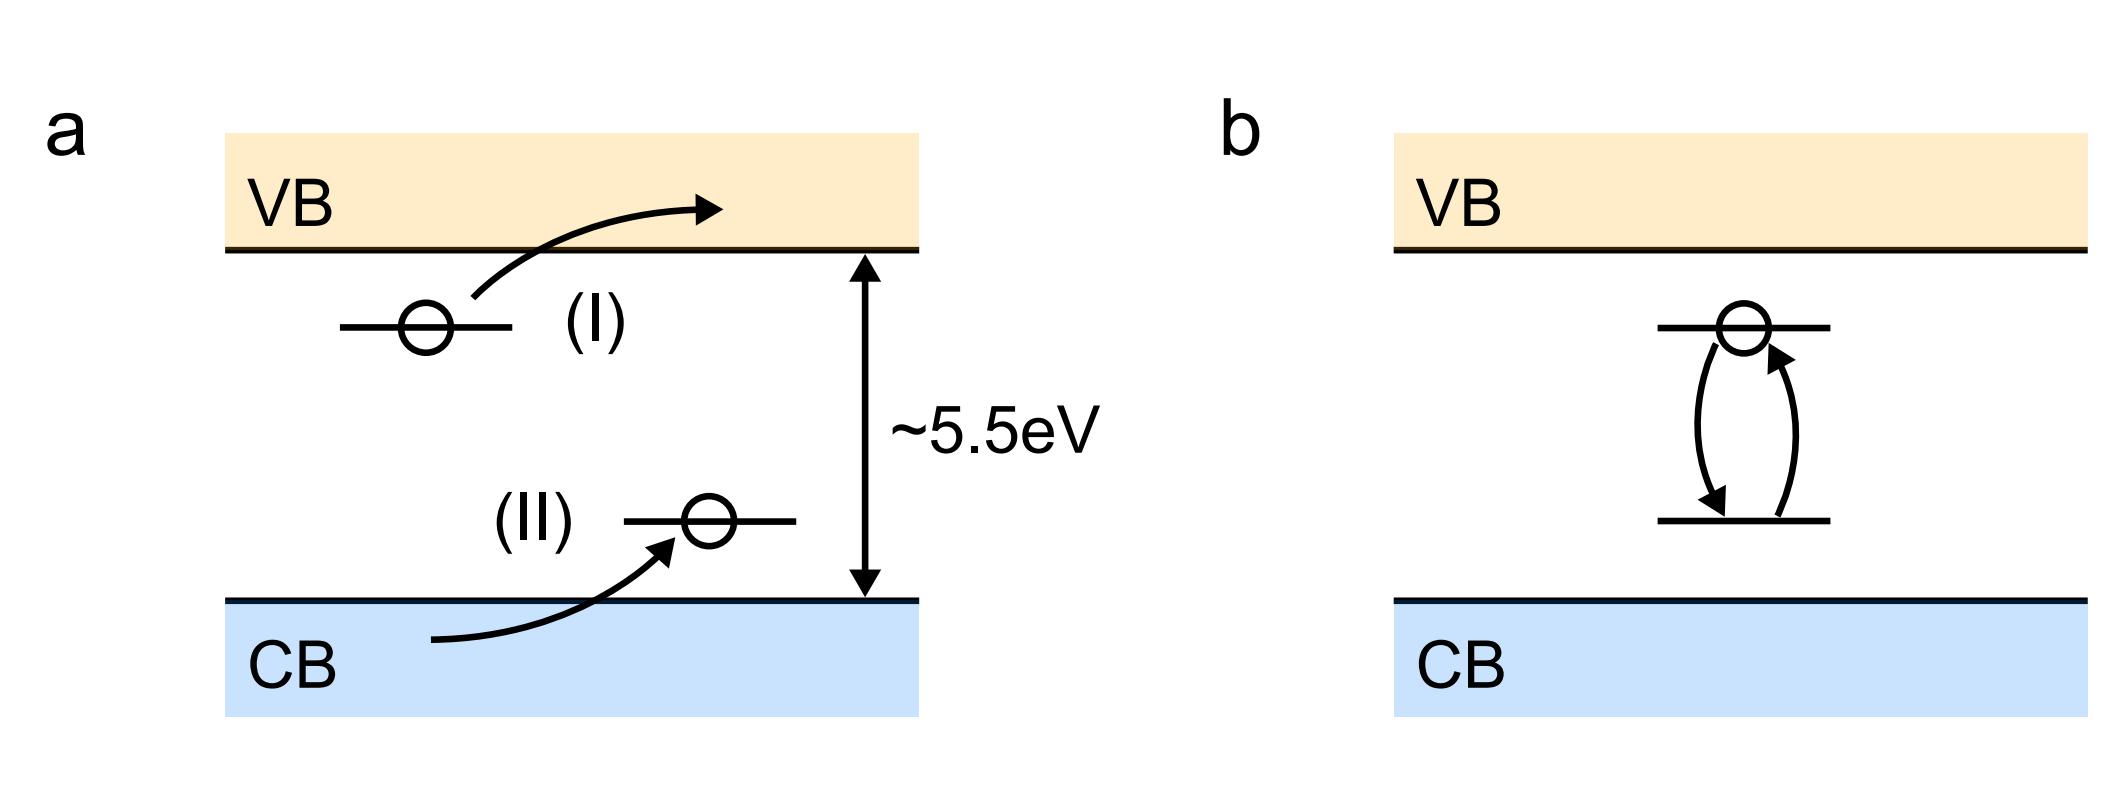
\includegraphics[width=0.9\textwidth]{figures/Chapter 1/Optical Transition.png}
  \caption[含有缺陷的金刚石晶体的电子能级结构]{含有缺陷的金刚石晶体的电子能级结构。(a)带隙之间的施主和受主能级会使电子发生在价带和缺陷能级(\uppercase\expandafter{\romannumeral1})或缺陷能级和导带(\uppercase\expandafter{\romannumeral2})之间的光学跃迁。(b)电子在施主和受主能级之间的光学跃迁。}
  \label{fig: Optical Transition}
\end{figure}

\section{金刚石中氮-空位色心的结构和性质}

由于本文主要是围绕金刚石中氮-空位色心的各种性质进行讨论,并结合实验对其进行表征,因此本节将对其结构和性质进行详细的介绍。氮-空位色心不仅仅存在于金刚石中,还可能存在于其他的半导体晶体如碳化硅(SiC)之中,而本文所有的讨论和实验都是基于金刚石中的氮-空位色心,出于方便起见,后文叙述中所有的“NV色心”和“NV Center”都是指金刚石中的氮-空位色心\cite{von2015identification, csore2017characterization}。

\subsection{NV Center的结构}
NV Center是金刚石中最常见的色心之一,其结构如图1.4所示,它是由一个氮原子替位原本的碳原子和邻近的一个空位缺陷组成的复合缺陷结构,其晶格结构中的空位缺陷是金刚石晶格中最常见的缺陷,而氮原子是金刚石中最常见的杂质之一,因此NV Center是金刚石中最常见的色心之一。我们定义NV Center的轴向为氮原子和空位中心的连线,也就是晶胞的[111]轴向。氮原子和围绕空位的三个碳原子形成了高度对称的$C_{3v}$对称性结构,这种结构使得NV Center的晶体结构具有很高的对称性(其结构对称性见图1.5),从而使得NVCenter的电子结构和光学性质具有很高的稳定性。

\begin{figure}
  \centering
  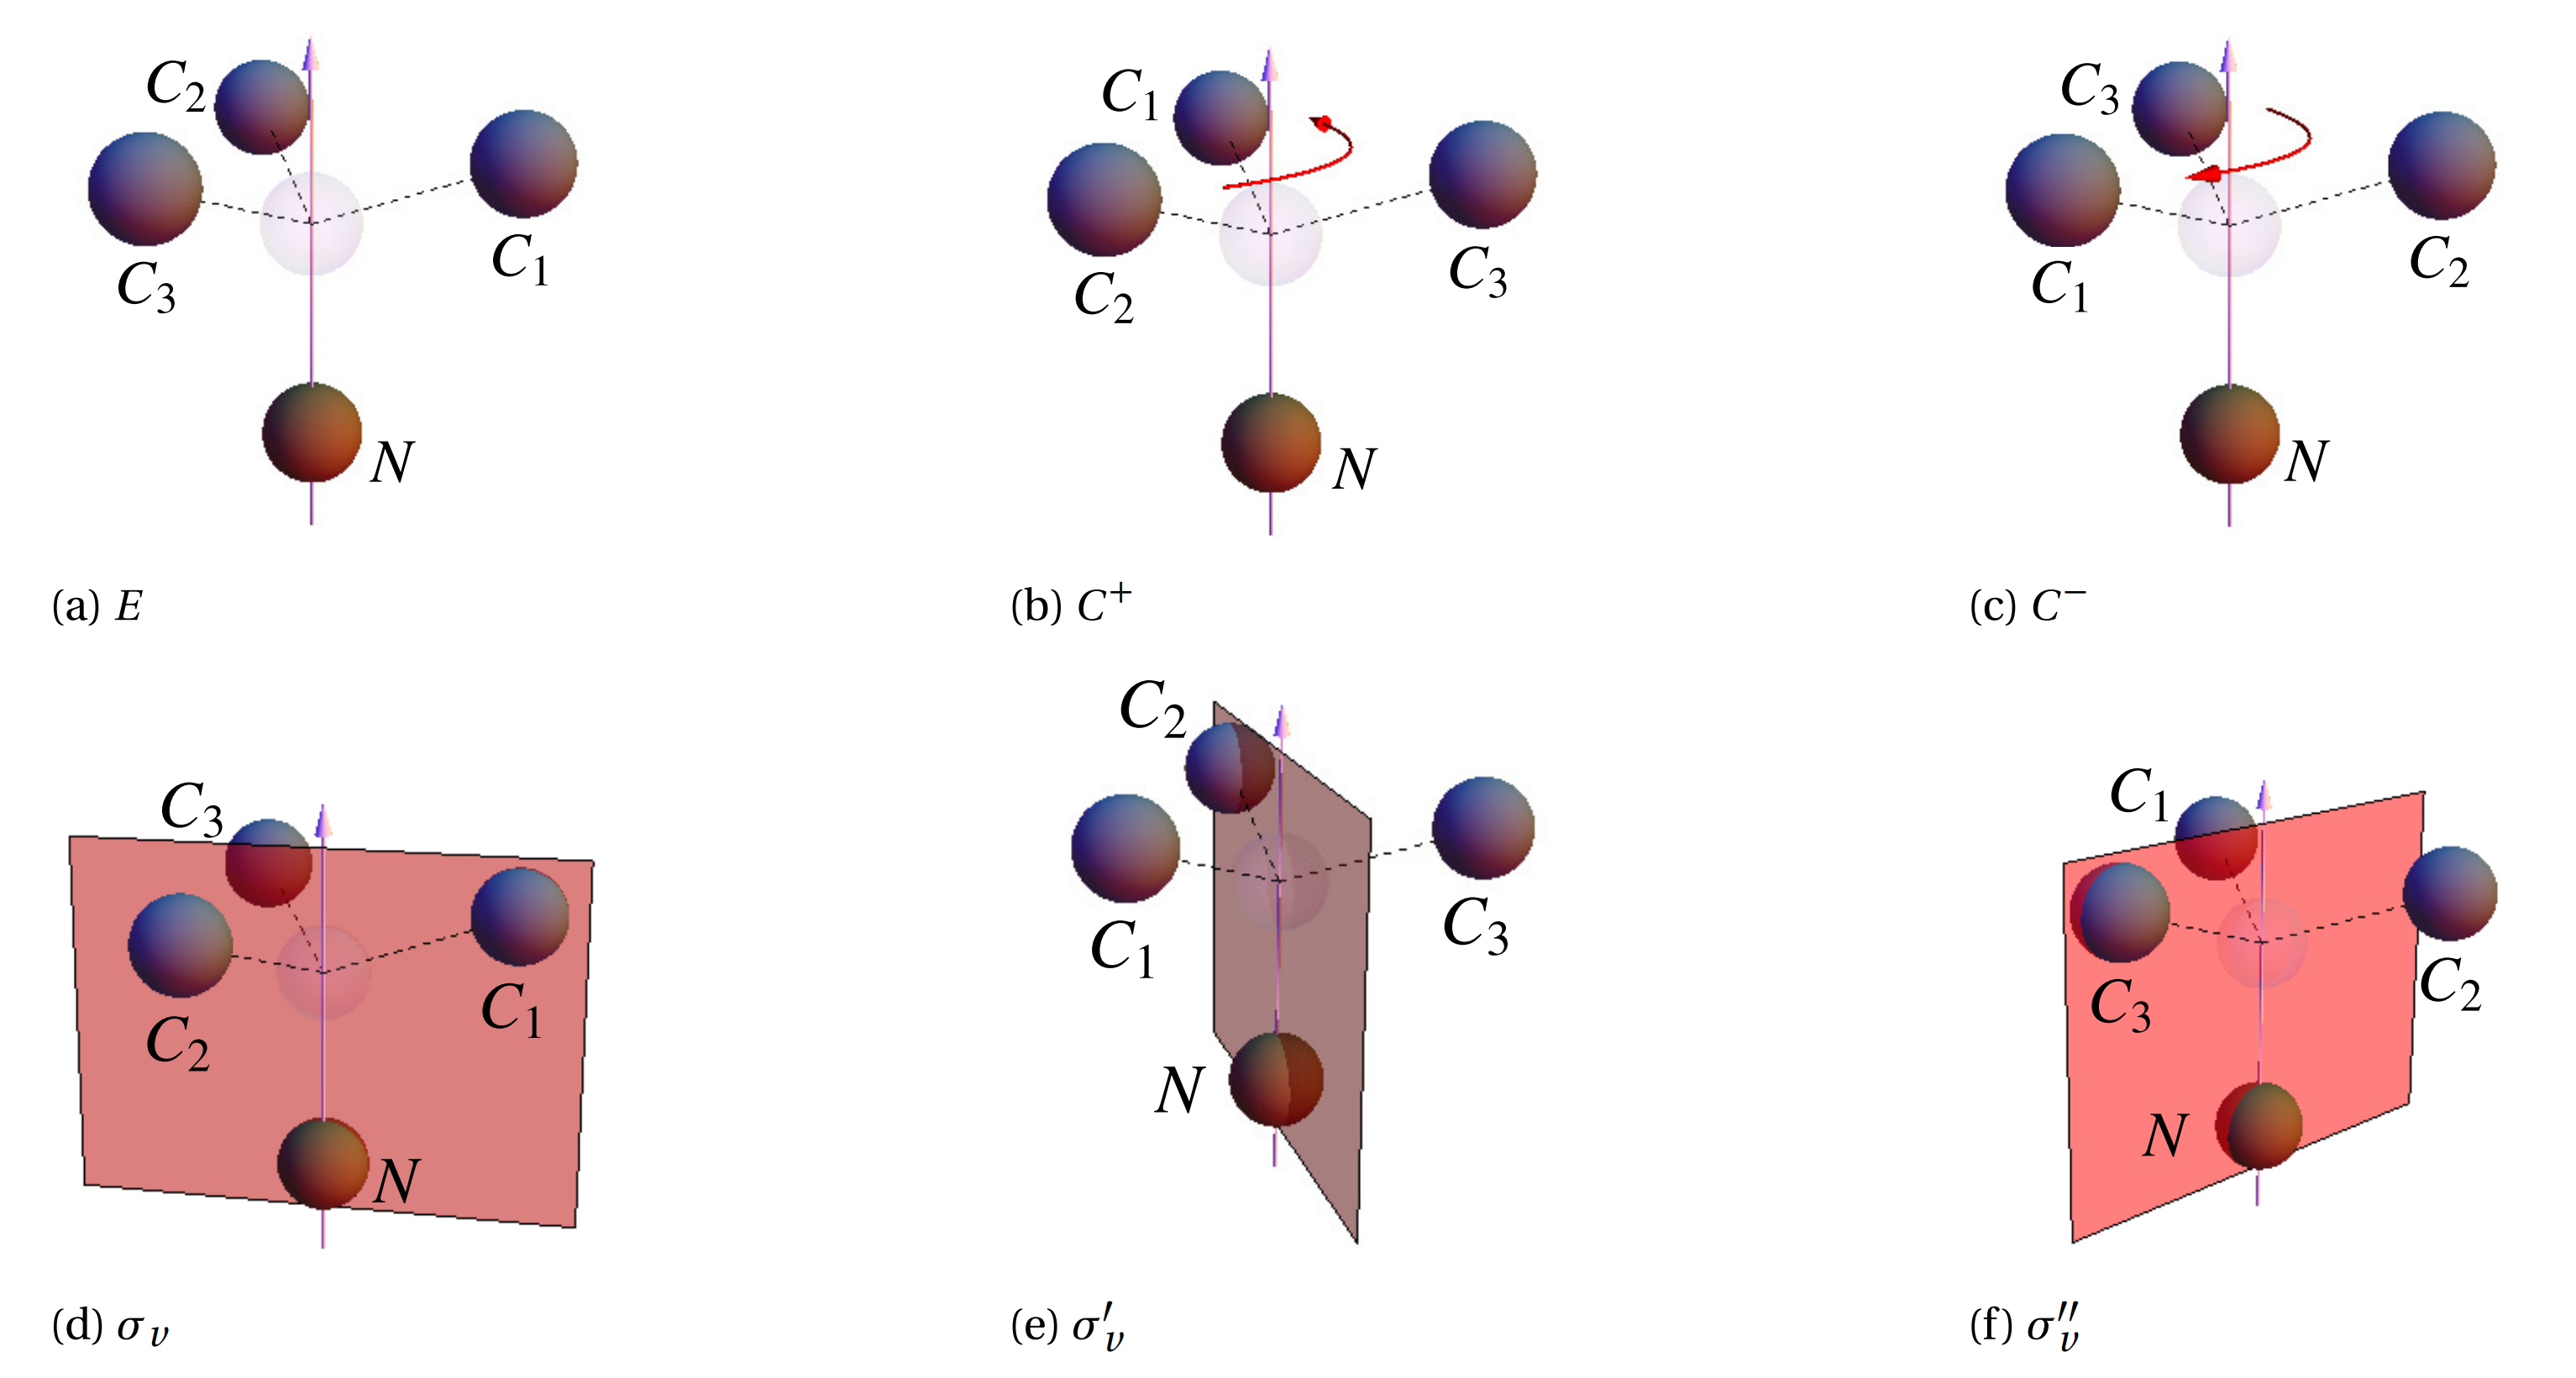
\includegraphics[width=1.0\textwidth]{figures/Chapter 1/NV Symmetry.png}
  \caption[金刚石的C$_{3v}$对称性群结构]{金刚石的C$_{3v}$对称性群结构,氮原子和围绕空位(中心半透明标识)的三个碳原子沿着[111]轴旋转对称,同时也沿着每个碳原子分别和空位、氮原子组成的平面镜像对称。}
  \label{fig: NV Symmetry}
\end{figure}

近十几年来,随着半导体的工艺进步和计算机的广泛运用,人们开发了许多强有力的科学计算工具,通过基于密度泛函理论(Density Functional Theory, DFT)第一性原理(First-principles),利用杂化泛函Heyd-Scuseria-Ernzerhof (HSE06)算法可以较为准确地得到NV Center的自旋密度(Spin Density)和带隙中各能级的电荷密度(Charge Density),如图1.6所示,可以看到NV$^-$的自旋密度和带隙中各个缺陷能级的电荷密度都是围绕$C_{3v}$旋转对称\cite{zou2023influence}。

\begin{figure}
  \centering
  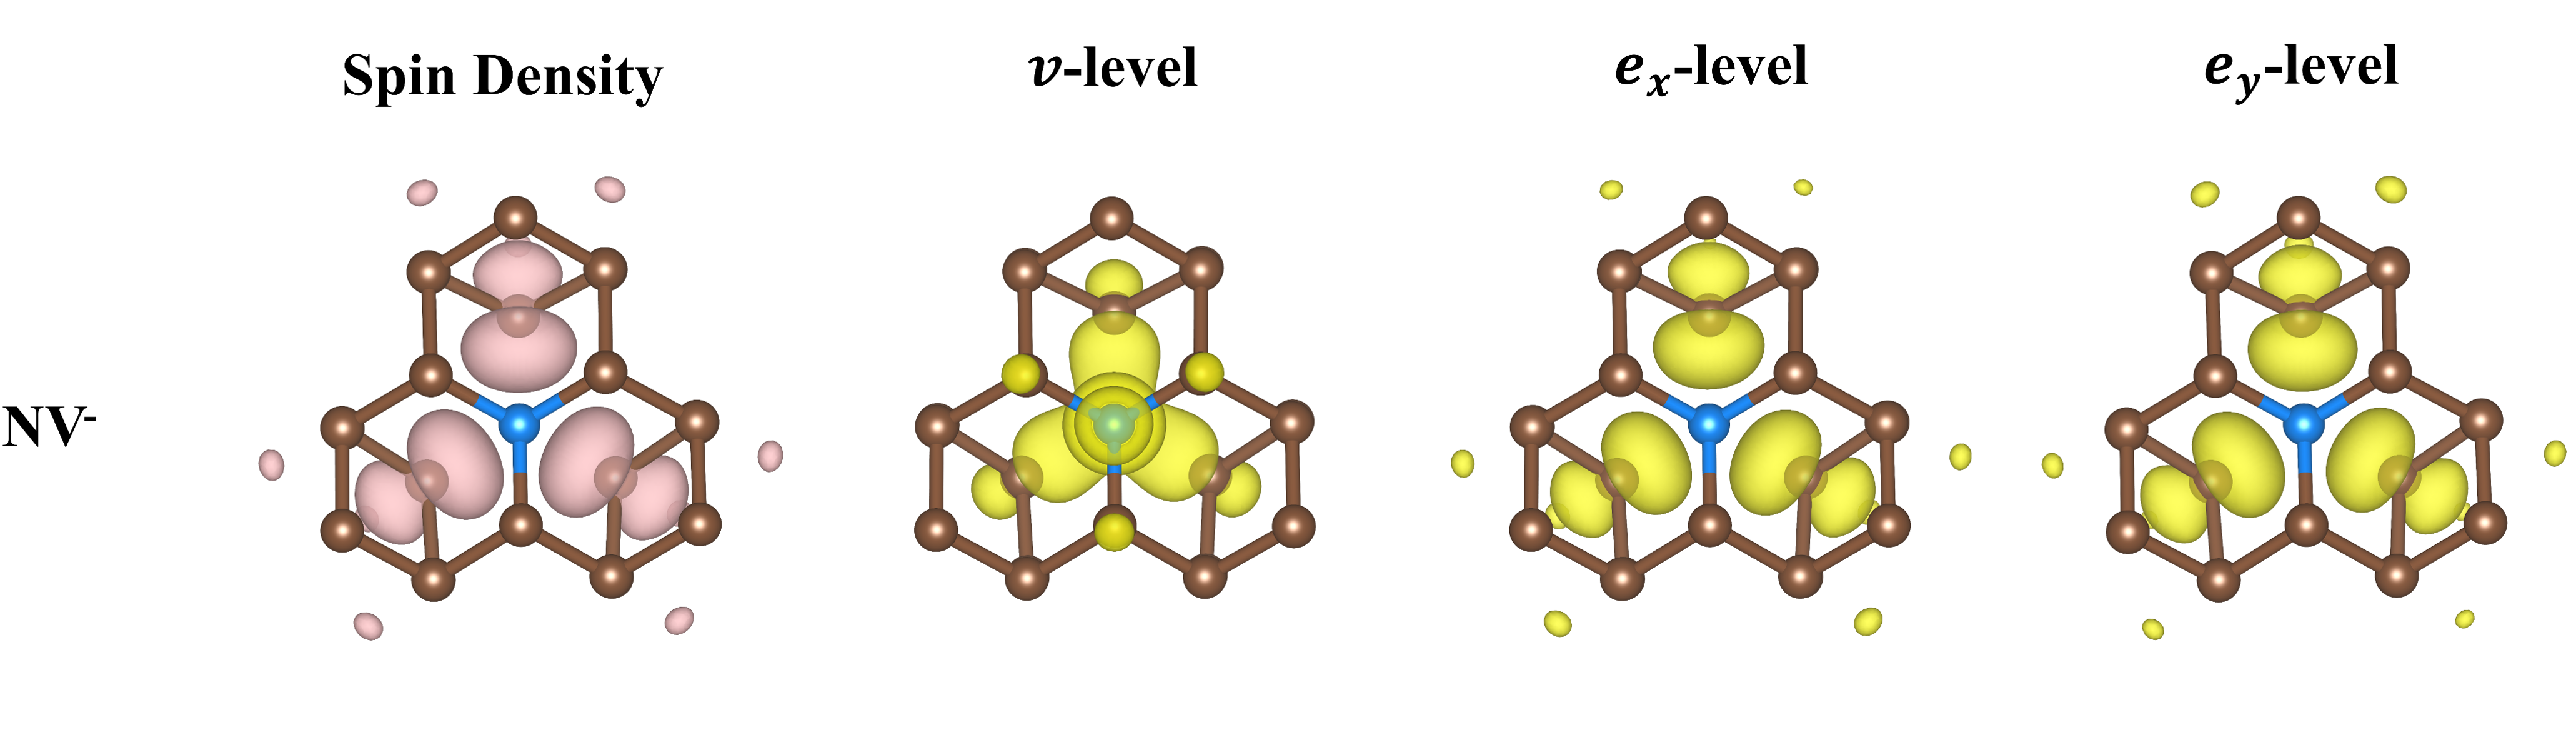
\includegraphics[width=1.0\textwidth]{figures/Chapter 1/Spin and Charge Density.png}
  \caption[基态NV$^-$的自旋密度和带隙中各个缺陷能级的电荷密度分布]{基态NV$^-$的自旋密度和带隙中各个缺陷能级的电荷密度分布,其中蓝色的原子为氮原子,棕色的原子为碳原子,视角沿$C_{3v}$轴的[-1 -1 -1]方向,粉红色的区域为自旋密度分布,淡黄色的区域为电荷密度分布,isovalue的设置为0.0078 \unit{e\per\bohr\cubed}}
  \label{fig: Spin and Charge Density}
\end{figure}

由于氮元素是元素周期表上第五主族的元素,所以其外围电子层中有五个价电子,其中三个电子和周围三个碳原子结合形成共价键,剩余两个电子和空位周围的三个碳原子上剩余的一个电子共五个电子形成了中性的NV CenterNV$^0$,因此五个电子形成的自旋系统有一个孤立的电子自旋,所以NV$^0$的电子自旋量子数$S=\frac{1}{2}$。在实验上已经发现的NV Center的两种稳定的电荷态,中性的NV$^0$和带负电的NV$^-$,其中NV$^-$的电子自旋量子数$S=1$ \cite{waldherr2011dark,aslam2013photo,dolde2014nanoscale}。NV Center的电荷态取决于其周围的环境状态,比如附近存在的杂质、缺陷、电场,或者周围的施主、受主能级等,更进一步地,取决于整个金刚石体系的费米能级(Fermi Level,$E_F$)\cite{doherty2013nitrogen}。在金刚石中,NV Center的电荷态可以通过光学方法进行调控,比如通过激光光子的吸收和发射,可以使NV Center的电荷态在NV$^0$和NV$^-$之间进行转换\cite{doi2016pure,siyushev2013optically,shields2015efficient}。通常情况下,NV Center可能并不会处于某种特定单一的状态,而是在两个电荷态之间不断地切换。在NV Center的电荷态切换的过程中,其电子自旋态也会发生变化,这种变化可以通过光学方法进行探测和读出,从而可以对NV Center的电荷态进行探测,这也是本文主要聚焦的问题。

对于NV Center的两种电荷态NV$^0$和NV$^-$而言,我们最主要的区分方式就是其光谱特征的不同,两种电荷态在零声子线处(zero phonon line, ZPL)都有较为强烈的光学跃迁现象。零声子线是指在光谱中的一种特殊峰值或能级跃迁,其特点是在跃迁过程中不伴随着声子(晶格振动)的吸收或发射,此状态下的能级跃迁是非常干净和锐利的,不受热振动的影响,通常情况下接近绝对零度的时候,声子的振动作用极其微弱,晶体的大部分光学跃迁都接近于ZPL的波长。零声子线通常表示了一个非常纯净的能级跃迁,因为它不受晶格振动引起的能级展宽的影响。如图1.7所示,NV$^-$的零声子线位于637 nm处,而NV$^0$的零声子线位于575 nm处。在室温条件下,由于声子振动不可避免的影响,零声子线总会伴随着较强的声子边带(phonon sidebands)效应,导致NV Center的光谱出现展宽现象,而不是在ZPL处出现极其尖锐突出的峰值。

\begin{figure}
  \centering
  \includegraphics[width=1.0\textwidth]{figures/Chapter 1/NV Spectrum.png}
  \caption[NV Center在不同电荷态的时候的光谱图象]{NV Center在不同电荷态的时候的光谱图象,其中红色的线为NV$^-$的光谱,蓝色的线为NV$^0$的光谱,NV$^-$的零声子线位于637 nm处,NV$^0$的零声子线位于575 nm处。}
  \label{fig: NV Spectrum}
\end{figure}

\section{电子能级结构}

\subsection{NV$^-$的电子能级结构}
对于我们最为关注的NV$^-$而言,其电子的能级结构可以用几个简单的三能级系统模型来描述,这个模型包括基态(ground state, GS)三重态(triplet)$^3A_2$(如图1.8a)、激发态(excited state, ES)三重态$^3E$(如图1.8b)和中间自旋单态(singlet state)。NV Center的负电荷状态NV$^-$是中性的NV$^0$捕获了一个电子形成的一个六电子缺陷能级结构,电子自旋量子数$S=1$的体系,这个结构可以通过各种方式在理论上进行模拟和验证,包括密度泛函理论、群论等方法\cite{lenef1996electronic,goss1997comment, maze2011properties, hossain2008ab, gali2009theory}。其中群论是一个非常强大且实用的工具,A. lenef和S. C. Rand在1996年的时候就通过群论预测了NV Center中的电子能级结构,其中较低的两个能级($a_1(1), a_2(2)$)有$a_1$对称性,较高的两个能级($e_x, e_y$)则在能量上退化兼并到关于$e$对称\cite{lenef1996electronic}。这些结论在后来人们拥有了超级计算机进行大规模密度泛函理论从头算(ab initio)的模拟的各项研究中被反复广泛的验证其可靠性和准确性\cite{gali2009theory, zou2023influence}。

在GS和ES的时候,三重态能级会发生零场劈裂(zero field splitting, ZFS)的现象,出现两个可以分辨的自旋能级$m_s=0$和$m_s=±1$,其中$m_s$为电子磁量子数。在GS的时候,其GS-ZFS的劈裂宽度大约为2870 \unit{\MHz},这使得其基态的自旋状态可以被微波(microwave, MW)所调控;而在ES的时候,其ES-ZFS约为GS-ZFS的一半,大概为1420 \unit{\MHz} \cite{gruber1997scanning,neumann2009excited}。

对于NV$^-$而言,缺陷能级中一共有六个价电子,在$^3A_2$基态的时候,$a_1(1), a_2(2)$能级都是被电子完全占据的,剩下的两个电子分别占据了$e_x, e_y$这两个能量较高的能级,便构成了$S=1$的自旋三重态。在$^3A_2$和$^3E$能级之间,电子可以发生较为明显的ZPL偶极跃迁,其在室温条件下,$a_2(2)$能级中自旋向下的电子吸收532 nm的绿光光子跃迁到被激发到$e_x$能级,然后退激发释放637 nm (1.945 \unit{\eV})的红光光子从而回到$^3A_2$基态,如图1.8c所示。值得注意的是,在室温条件下,电子从$^3E$能级退激发到基态的过程中,有一部分情况会不可避免的和晶体声子产生相互作用,通过系统间交叉(intersystem crossing, ISC),从自旋单态的声子边带退激发到$^3A_2$,这个过程中不会辐射出可见光,如图1.8c所示。

\begin{figure}
  \centering
  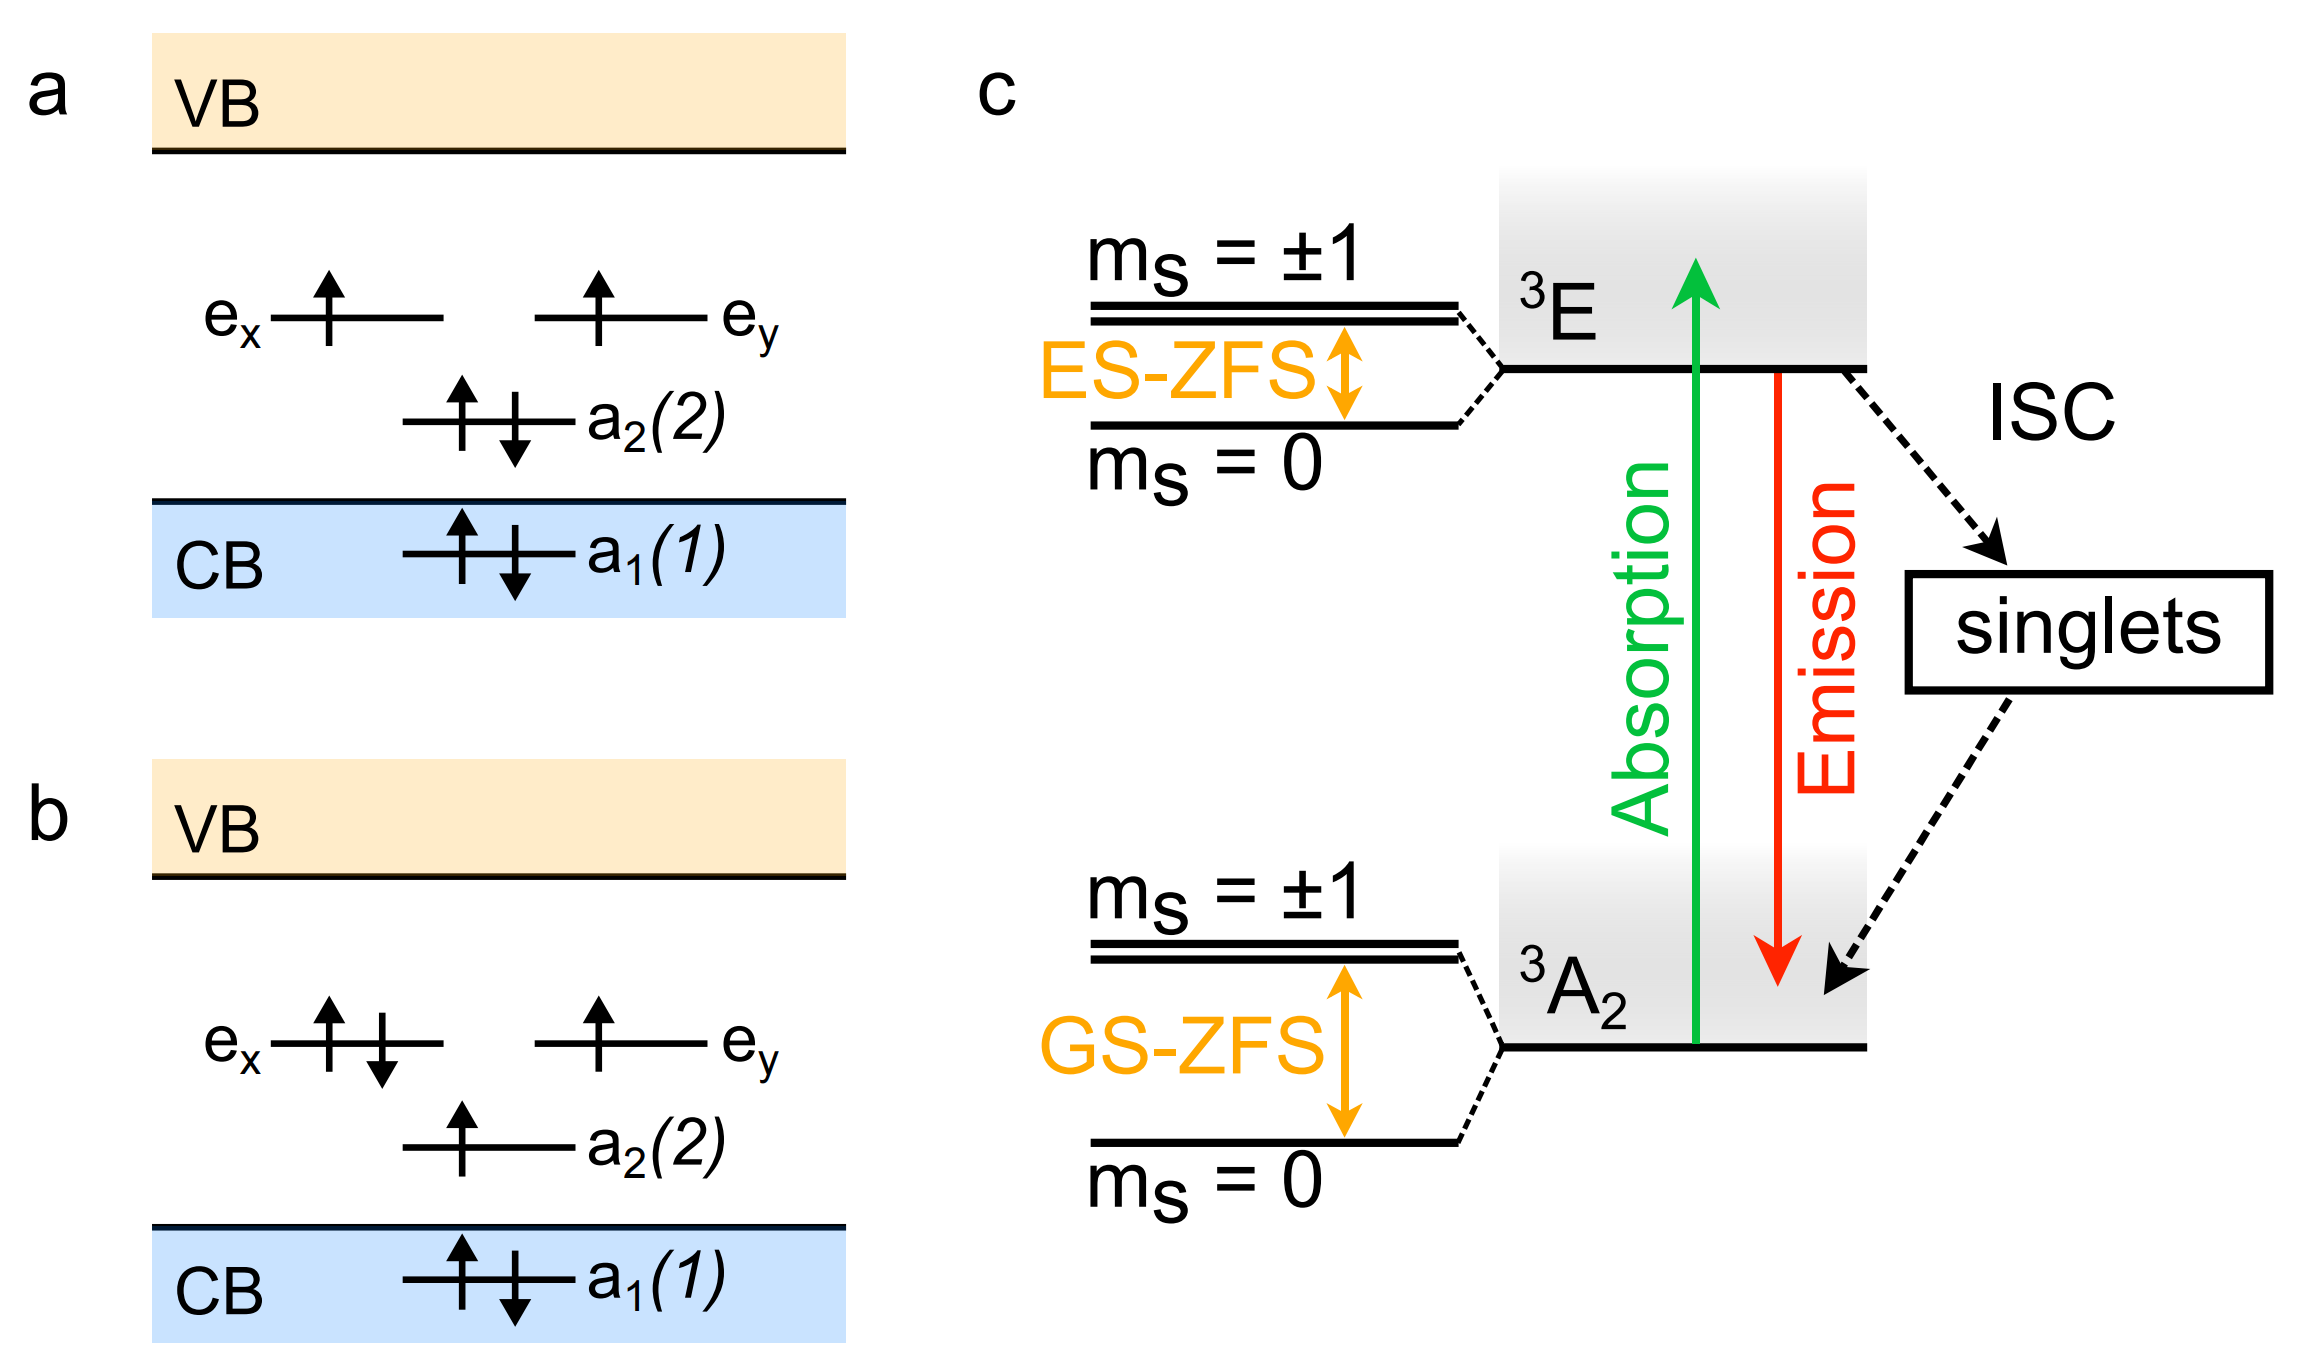
\includegraphics[width=1.0\textwidth]{figures/Chapter 1/Electronic Structure.png}
  \caption[NV$^-$的电子能级结构示意图]{NV$^-$的电子能级结构示意图,展示了带隙中间的缺陷能级:(a)$^3A_2$基态;(b)$^3E$激发态;(c)自旋三重态和ZPL跃迁过程,以及在自旋单态下的声子边带的ISC作用。}
  \label{fig: NV Spectrum}
\end{figure}

需要注意的一点是,图1.8中所展示的NV Center的电子能级结构仅仅是一个简单的示意图,更加详细的细节,比如自旋单态ISC过程的能级结构、电子和氮核自旋之间超精细相互作用(hyperfine interaction)在这里并没有详细的给出,这些内容会在后续的章节中有所涉及。

由于金刚石的德拜温度(Debye temperature)较高,所以声子态密度在环境室温的情况下较小,因此NV Center有着较低的电子-声子耦合性,从而有着较长的$T_1$弛豫时间\cite{koizumi2008physics}。较长的$T_1$时间与金刚石中较弱的自旋-轨道作用密切相关,其使得NV自旋态之间产生微小的混合状态,这些自旋态又与电子-声子相互作用发生耦合,从而使得NV自旋态发生弛豫。


\section{各节一级标题}
我是内容

\subsection{各节二级标题}
你是内容

\subsubsection{各节三级标题}
他是内容

\paragraph{四级标题}
内容内容

\subparagraph{五级标题}
内容内容

\section{字体样式}
宋体\quad \textbf{粗体}\quad \textit{斜体}\quad \textbf{\textit{粗斜体}}。

{\heiti 黑体\quad \textbf{粗体}\quad \textit{斜体}\quad \textbf{\textit{粗斜体}}}。

{\fangsong 仿宋\quad \textbf{粗体}\quad \textit{斜体}\quad \textbf{\textit{粗斜体}}}。

{\kaishu 楷书\quad \textbf{粗体}\quad \textit{斜体}\quad \textbf{\textit{粗斜体}}}。

Serif\quad \textit{Italic}\quad \textbf{Bold}\quad \textbf{\textit{BoldItalic}}

{\sffamily Sans\quad \textit{Italic}\quad \textbf{Bold}\quad \textbf{\textit{BoldItalic}}}

{\ttfamily Mono\quad \textit{Italic}\quad \textbf{Bold}\quad \textbf{\textit{BoldItalic}}}

\end{document}